\documentclass[12pt]{article}

\usepackage[margin=1in]{geometry}
\usepackage{amsmath}
\usepackage{amssymb}
\usepackage{graphicx}
\usepackage{float}
\usepackage{hyperref}
\usepackage{booktabs}
\usepackage{caption}
\usepackage{subcaption}
\usepackage{enumitem}
\usepackage{fancyhdr}
\usepackage{setspace}
\usepackage{titlesec}
\usepackage{cite}
\usepackage{listings}
\usepackage{xcolor}
\usepackage{tikz}
\usetikzlibrary{shapes.geometric, arrows.meta, positioning, fit, backgrounds, calc}

\pagestyle{fancy}
\fancyhf{}
\rhead{ECE 445 --- Individual Progress Report}
\lhead{Max Beach}
\rfoot{Page \thepage}

\lstset{
  basicstyle=\ttfamily\small,
  keywordstyle=\color{blue},
  commentstyle=\color{gray},
  breaklines=true,
  frame=single
}

\title{
  \textbf{ECE 445 Individual Progress Report} \\
  \large BetaSpray: Automated Climbing Route Annotation System \\[0.5em]
  \normalsize Max Beach \\
  University of Illinois Urbana-Champaign \\
  \today
}
\date{}

\begin{document}

\maketitle
\thispagestyle{fancy}

\tableofcontents
\newpage

% ─────────────────────────────────────────────────────────────────
\section{Introduction}
% ─────────────────────────────────────────────────────────────────

BetaSpray is an automated climbing route annotation system that scans a climbing
wall using a camera, detects the locations of climbing holds via computer vision,
and then directs laser gimbals to highlight specific holds that form a climber's
chosen route.  The system is built around an ESP32-S3 microcontroller running a
custom firmware stack written in C using the ESP-IDF framework.

The three primary subsystems are:
\begin{enumerate}
  \item \textbf{Vision / Camera Subsystem} --- An OV5640 5\,MP camera connected
        over a DVP parallel interface, supported by an on-device calibration
        pipeline and a tiled high-resolution capture mode for wall scanning.
  \item \textbf{Projection Subsystem} --- Four two-axis servo gimbals, each
        carrying a laser module, driven by PWM signals generated via the ESP32-S3
        LEDC peripheral.
  \item \textbf{User Interface Subsystem} --- A Wi-Fi soft-AP HTTP server that
        exposes REST endpoints for route upload, capture triggering, and live
        control.
\end{enumerate}

\begin{figure}[H]
\centering
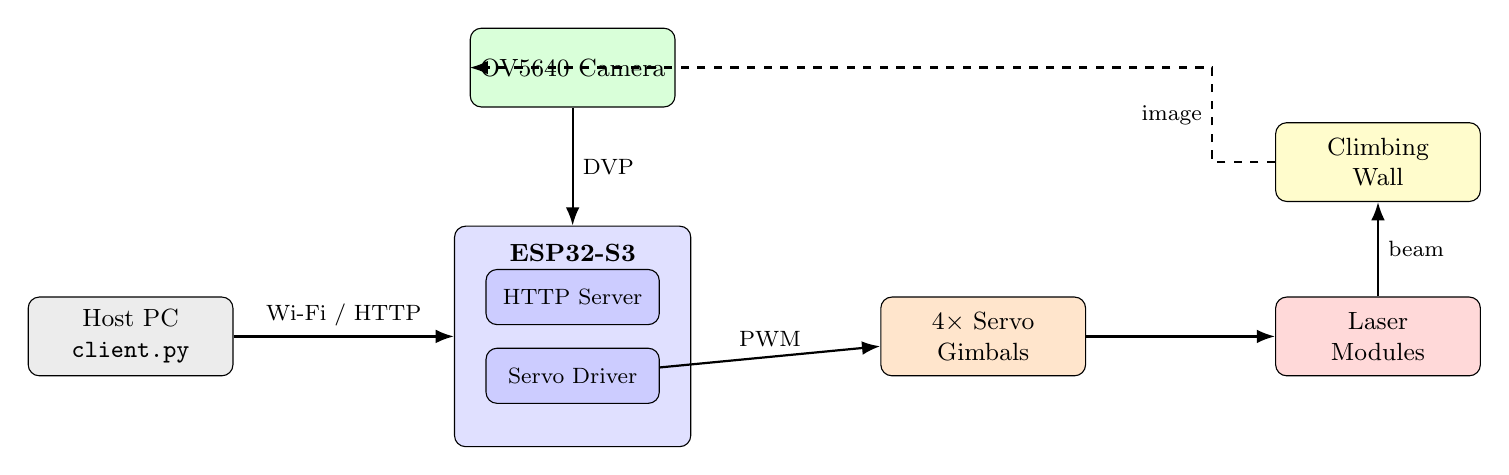
\begin{tikzpicture}[
  box/.style={draw, rounded corners=4pt, minimum width=2.6cm, minimum height=1cm,
              align=center, font=\small},
  arr/.style={-{Latex}, thick},
  node distance=1.1cm and 2.2cm
]
  % Host PC
  \node[box, fill=gray!15] (host) {Host PC \\ \texttt{client.py}};

  % ESP32-S3
  \node[box, fill=blue!12, right=2.8cm of host, minimum width=3.0cm, minimum height=2.8cm]
    (esp) {};
  \node[font=\small\bfseries] at (esp.north) [yshift=-0.35cm] {ESP32-S3};

  % Internal ESP nodes
  \node[box, fill=blue!20, minimum width=2.2cm, minimum height=0.7cm,
        font=\footnotesize] at ([yshift=0.5cm]esp.center) (http) {HTTP Server};
  \node[box, fill=blue!20, minimum width=2.2cm, minimum height=0.7cm,
        font=\footnotesize] at ([yshift=-0.5cm]esp.center) (servo_fw) {Servo Driver};

  % Camera
  \node[box, fill=green!15, above=1.5cm of esp] (cam) {OV5640 Camera};

  % Servo gimbals
  \node[box, fill=orange!20, right=2.4cm of esp] (gimbal) {4$\times$ Servo \\ Gimbals};

  % Laser
  \node[box, fill=red!15, right=2.4cm of gimbal] (laser) {Laser \\ Modules};

  % Wall
  \node[box, fill=yellow!20, above=1.2cm of laser] (wall) {Climbing \\ Wall};

  % Arrows
  \draw[arr] (host) -- node[above,font=\footnotesize]{Wi-Fi / HTTP} (esp);
  \draw[arr] (cam) -- node[right,font=\footnotesize]{DVP} (esp);
  \draw[arr] (servo_fw) -- node[above,font=\footnotesize]{PWM} (gimbal);
  \draw[arr] (gimbal) -- (laser);
  \draw[arr] (laser) -- node[right,font=\footnotesize]{beam} (wall);
  \draw[arr, dashed] (wall.west) -- ++(-0.8,0) |- node[left,font=\footnotesize,pos=0.25]{image} (cam.west);
\end{tikzpicture}
\caption{BetaSpray system block diagram.  The ESP32-S3 acts as the central
  controller: it captures wall images from the OV5640 over DVP, runs the tiling
  and (planned) DoG hold-detection pipeline, accepts route selections from the
  host PC over Wi-Fi, and drives the servo gimbals via PWM to point laser modules
  at the selected holds.}
\label{fig:block}
\end{figure}

My individual contributions span all three subsystems but are concentrated in
vision software and PCB design/layout for the power delivery infrastructure.
Specifically, I have:

\begin{itemize}
  \item Designed and laid out the servo power subsystem PCB in KiCad,
        including bulk capacitance sizing for the 5\,V servo rail.
  \item Contributed to the laser diode power system PCB layout.
  \item Soldered and assembled the ESP32-S3 development board used as our
        primary validation target.
  \item Written the servo firmware driver, including the GPIO pin assignment
        that resolved a camera-servo conflict, and hardware fade/hold logic.
  \item Performed servo reliability and repeatability testing, quantifying
        positional drift and variability under repeated actuation.
  \item Tuned the servo drive profile to reduce mechanical jerk and
        momentum overshoot.
  \item Implemented camera lens-distortion documentation and calibration
        tooling (\texttt{calibrate\_camera.py}).
  \item Implemented a tiled high-resolution image capture mode that
        overcomes the dev board's DRAM limitations, enabling full-resolution
        wall scans for downstream computer-vision testing.
\end{itemize}

Teammate Ingi Helgason owns the Difference-of-Gaussian (DoG) blob detector and
the power subsystem schematic; teammate Prakhar Gupta owns the vision-subsystem
schematic and firmware bringup for Wi-Fi, HTTP, and FatFS.  My tiling work
directly feeds Ingi's DoG pipeline: the stitched high-resolution image is the
input to hold detection.

The DoG detector is the computer-vision algorithm used to locate climbing holds
in the wall image.  It works by blurring the image with Gaussian filters at
multiple scales $\sigma_0, \sigma_1, \ldots$ and then subtracting adjacent
blurred images (\emph{Difference of Gaussians}).  The resulting difference images
approximate the Laplacian of Gaussian --- a well-known blob detector --- and
produce strong responses at image locations where the intensity changes at a
scale that matches the filter spacing.  Climbing holds appear as roughly circular
blobs in the image; the DoG responses peak at their centres.  Local maxima in
the difference images that exceed a contrast threshold are collected as
\emph{keypoints}, then de-duplicated with non-maximum suppression (NMS) to
produce a final list of $(x, y)$ hold coordinates.  This algorithm was
implemented by Ingi in \texttt{differenceofgaussian.c} using four octaves and
three scales per octave, and runs on a host PC (gcc, libjpeg) using
images fetched from the ESP32-S3 via HTTP; on-device execution is planned
once the PSRAM-equipped PCB is available.

% ─────────────────────────────────────────────────────────────────
\section{Design}
% ─────────────────────────────────────────────────────────────────

\subsection{PCB Design --- Servo Power Subsystem}

\subsubsection{Schematic}

The servo power subsystem sheet was created in KiCad as a dedicated child sheet
(\texttt{servo\_subsystem}), keeping it separate from the top-level schematic for
clarity during review.  The sheet contains:

\begin{itemize}
  \item Eight SG90 servo connectors (four gimbals $\times$ two axes).
  \item The 5\,V servo supply rail, drawn directly from the USB-C input
        upstream of the LM3940IT-3.3 LDO.
  \item Bulk decoupling capacitors on the 5\,V servo rail (see
        Section~\ref{sec:bulk_cap}).
  \item PWM signal routing from the ESP32-S3 GPIOs through the connector bank.
\end{itemize}

\begin{figure}[H]
  \centering
  \fbox{\parbox{0.7\textwidth}{\centering\vspace{2cm}
    \textit{[PLACEHOLDER: KiCad servo\_subsystem schematic screenshot]}
  \vspace{2cm}}}
  \caption{Servo power and control subsystem schematic.}
  \label{fig:servo_schematic}
\end{figure}

\subsubsection{Bulk Capacitance Sizing}
\label{sec:bulk_cap}

The SG90 servo draws significant transient current when it begins to move.
Table~\ref{tab:sg90_current} summarises the datasheet current figures.

\begin{table}[H]
  \centering
  \caption{SG90 current draw at nominal operating voltages.}
  \label{tab:sg90_current}
  \begin{tabular}{lcc}
    \toprule
    Condition & 4.8\,V & 6.0\,V \\
    \midrule
    No-load (holding) & $\sim$10\,mA & $\sim$15\,mA \\
    Moderate load (moving) & 100--200\,mA & 150--250\,mA \\
    Stall (shaft blocked) & $\sim$650\,mA & $\sim$700\,mA \\
    \bottomrule
  \end{tabular}
\end{table}

With eight servos, a worst-case simultaneous slew draws up to $\sim$1.5\,A on
the 5\,V rail.  Without sufficient bulk capacitance, the resulting voltage droop
propagates through the LM3940IT-3.3 LDO and destabilises the 3.3\,V ESP32-S3
logic rail.

To hold the voltage droop $\Delta V$ below 200\,mV for a single servo stepping
from idle to load ($\Delta I \approx 200$\,mA, $\Delta t \approx 2$\,ms):

\begin{equation}
  C = \frac{I \,\Delta t}{\Delta V}
    = \frac{0.2\;\text{A} \times 0.002\;\text{s}}{0.2\;\text{V}}
    = 2000\;\mu\text{F}
  \label{eq:bulk_cap}
\end{equation}

Scaling for multiple simultaneous servo transitions, a value of 4700--10\,000\,$\mu$F
is warranted on the 5\,V servo rail, placed close to the connector bank.  The
LDO output also carries local decoupling (100\,$\mu$F + 100\,nF) to ride out
fast transients before they affect the ESP32-S3.

\subsubsection{PCB Layout}

\begin{figure}[H]
  \centering
  \fbox{\parbox{0.7\textwidth}{\centering\vspace{2cm}
    \textit{[PLACEHOLDER: KiCad PCB layout screenshot --- servo area]}
  \vspace{2cm}}}
  \caption{PCB layout showing servo connector bank and bulk capacitors.}
  \label{fig:pcb_layout}
\end{figure}

The layout is a two-layer board submitted for fabrication in March 2026.  Bulk
capacitors are placed immediately adjacent to the servo connector bank to
minimise inductive loop area on the high-current 5\,V rail.  Routing tracks were
added iteratively across several sessions, with the final Ver0 gerbers exported
and submitted.

\subsection{PCB Design --- Laser Diode Power System (Contribution)}

I contributed to the laser diode power system layout designed primarily by Ingi.
This involved reviewing the supply routing for the laser modules and ensuring the
layout was consistent with the overall board floor-plan.

\begin{figure}[H]
  \centering
  \fbox{\parbox{0.7\textwidth}{\centering\vspace{2cm}
    \textit{[PLACEHOLDER: PCB layout screenshot --- laser diode power area]}
  \vspace{2cm}}}
  \caption{Laser diode power subsystem PCB layout.}
  \label{fig:laser_layout}
\end{figure}

\subsection{Development Board Assembly}

The ESP32-S3-DevKitC-1 (N8 variant, no PSRAM) was hand-soldered and assembled
for use as the primary validation platform.  This includes all surface-mount
passive components and through-hole connectors used for early firmware bringup
prior to the custom PCB arriving from fabrication.

\subsection{Servo Firmware Driver}

\subsubsection{GPIO Pin Assignment}

During firmware bringup it was discovered that the originally assigned GPIO for
servo 0 conflicted with camera DVP data pins.  The pins were reassigned:
\texttt{SERVO\_PIN\_0} $\rightarrow$ GPIO1 (X-axis) and
\texttt{SERVO\_PIN\_1} $\rightarrow$ GPIO2 (Y-axis).
These pins are clear of all strapping, PSRAM SPI, UART, USB, and JTAG
constraints on the ESP32-S3-DevKitC-1.

\subsubsection{LEDC PWM Configuration}

The servo driver uses the ESP32-S3 LEDC peripheral:

\begin{itemize}
  \item Frequency: 50\,Hz (standard RC servo PWM)
  \item Resolution: 14-bit duty cycle counter
  \item Pulse range: 1\,ms (0°) to 2\,ms (180°)
\end{itemize}

The angle-to-duty conversion is a linear interpolation between the pulse width
extremes:

\begin{equation}
  D(\theta) = D_{\min} + \frac{\theta}{180°}\left(D_{\max} - D_{\min}\right)
  \label{eq:servo_duty}
\end{equation}

where $D_{\min}$ and $D_{\max}$ correspond to the 1\,ms and 2\,ms pulse widths
respectively at 50\,Hz with 14-bit resolution.

\subsubsection{Hardware Fade and Hold Logic}

A hardware fade + hold routine was implemented in \texttt{servo.c}: when a new
target angle is commanded, the LEDC timer smoothly ramps the duty cycle toward
the target (using the ESP-IDF LEDC fade API), then holds the final duty for a
configurable dwell period before releasing the PWM signal.  This reduces the
abrupt momentum seen when driving servos with a hard step.  The API is exposed
through \texttt{servo.h} and exercised in \texttt{main.c} at startup.

\subsection{Servo Drive Tuning}

Early tests showed the gimbals exhibited significant mechanical jerk and
momentum overshoot, causing the laser spot to oscillate around the target
position before settling.  The following parameters were tuned:

\begin{enumerate}
  \item \textbf{Fade step size} --- reducing the per-tick duty increment slows
        the angular velocity profile, limiting peak angular momentum.
  \item \textbf{Fade duration} --- increasing the total ramp time distributes
        the angular acceleration over a longer interval.
  \item \textbf{Hold duration} --- the post-move hold ensures the servo has
        fully settled before the PWM signal is removed; without this, the servo
        can drift back toward its rest position.
\end{enumerate}

\begin{figure}[H]
\centering
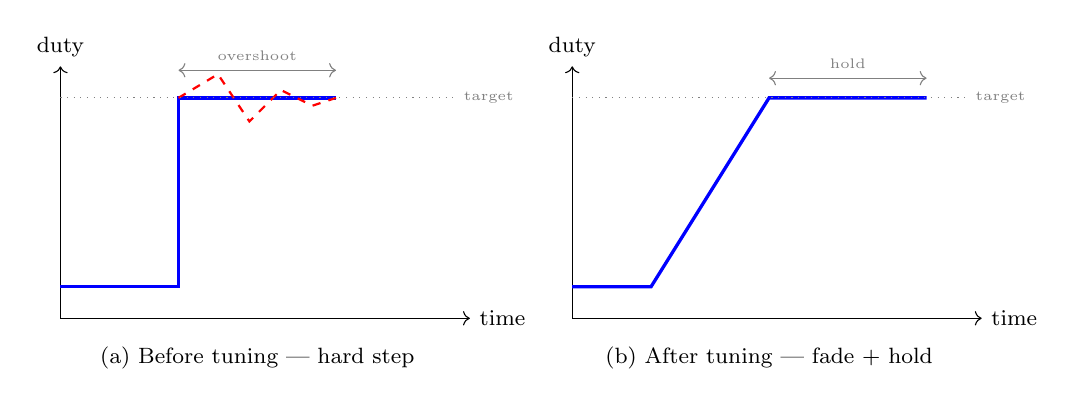
\begin{tikzpicture}
  \begin{scope}[xshift=0cm]
    % Axes
    \draw[->] (0,0) -- (5.2,0) node[right,font=\footnotesize]{time};
    \draw[->] (0,0) -- (0,3.2) node[above,font=\footnotesize]{duty};
    \node[font=\footnotesize] at (2.5,-0.5) {(a) Before tuning --- hard step};
    % Hard step profile
    \draw[blue, very thick] (0,0.4) -- (1.5,0.4) -- (1.5,2.8) -- (3.5,2.8);
    % Ringing / overshoot
    \draw[red, thick, dashed] (1.5,2.8) -- (2.0,3.1) -- (2.4,2.5) -- (2.8,2.9) -- (3.2,2.7) -- (3.5,2.8);
    \draw[<->, gray] (1.5,3.15) -- (3.5,3.15) node[midway,above,font=\tiny]{overshoot};
    % Target line
    \draw[dotted, gray] (0,2.8) -- (5,2.8) node[right,font=\tiny]{target};
  \end{scope}
  \begin{scope}[xshift=6.5cm]
    % Axes
    \draw[->] (0,0) -- (5.2,0) node[right,font=\footnotesize]{time};
    \draw[->] (0,0) -- (0,3.2) node[above,font=\footnotesize]{duty};
    \node[font=\footnotesize] at (2.5,-0.5) {(b) After tuning --- fade + hold};
    % Ramped profile
    \draw[blue, very thick] (0,0.4) -- (1.0,0.4) -- (2.5,2.8) -- (4.5,2.8);
    % Target line
    \draw[dotted, gray] (0,2.8) -- (5,2.8) node[right,font=\tiny]{target};
    % Hold brace
    \draw[<->, gray] (2.5,3.05) -- (4.5,3.05) node[midway,above,font=\tiny]{hold};
  \end{scope}
\end{tikzpicture}
\caption{Servo PWM duty-cycle profile before and after drive tuning.
  (a) A hard step immediately jumps to the target duty, causing mechanical
  overshoot and oscillation visible as ringing in the laser spot position.
  (b) The tuned fade profile ramps the duty linearly over a configurable
  interval and then holds, eliminating overshoot and allowing the servo to
  settle cleanly.}
\label{fig:servo_tune}
\end{figure}

\subsection{Camera Calibration and Lens Distortion Model}

\subsubsection{Distortion Model}

The OV5640 lens introduces radial and tangential distortion.  The standard
Brown-Conrady model is used:

\begin{equation}
  \begin{pmatrix} x' \\ y' \end{pmatrix}
  =
  \begin{pmatrix} x \\ y \end{pmatrix}
  \left(1 + k_1 r^2 + k_2 r^4 + k_3 r^6\right)
  +
  \begin{pmatrix}
    2p_1 xy + p_2(r^2 + 2x^2) \\
    p_1(r^2 + 2y^2) + 2p_2 xy
  \end{pmatrix}
  \label{eq:distortion}
\end{equation}

where $(x, y)$ are normalised image coordinates, $r^2 = x^2 + y^2$,
$k_1, k_2, k_3$ are radial distortion coefficients, and $p_1, p_2$ are
tangential distortion coefficients.  The calibrated coefficients are stored in
\texttt{conf.h} as compile-time constants.

\subsubsection{Calibration Procedure}

The script \texttt{calibrate\_camera.py} performs standard checkerboard-based
intrinsic calibration using OpenCV:

\begin{enumerate}
  \item Capture $N \geq 15$ frames of a known checkerboard pattern at varied
        orientations.
  \item Detect sub-pixel corner locations using \texttt{cv2.cornerSubPix}.
  \item Solve for the intrinsic matrix $\mathbf{K}$ and distortion vector
        $\mathbf{d}$ using \texttt{cv2.calibrateCamera}.
  \item Write the resulting coefficients into \texttt{conf.h}.
\end{enumerate}

A key constraint is that the N8 dev board has no PSRAM, so reliable multi-frame
capture for calibration requires careful frame buffering.  The final PCB
(ESP32-S3FH4R2, N16R8 with 8\,MB PSRAM) will remove this limitation.

\begin{figure}[H]
  \centering
  \fbox{\parbox{0.7\textwidth}{\centering\vspace{2cm}
    \textit{[PLACEHOLDER: Example checkerboard calibration image captured from
    OV5640]}
  \vspace{2cm}}}
  \caption{Sample calibration frame with detected corner overlay.}
  \label{fig:calibration}
\end{figure}

\subsection{Tiled High-Resolution Image Capture \textnormal{\textit{(work in progress)}}}

\subsubsection{Motivation}

The OV5640 sensor has an active array of $2592 \times 1944$ pixels.  A full
UXGA ($1600 \times 1200$) or higher frame requires tens of megabytes of
contiguous RAM --- well beyond the $\sim$320\,KB DRAM available on the N8 dev
board.  To enable high-resolution wall scans for image-recognition testing
without waiting for the PSRAM-equipped PCB, a tiling strategy was designed.

\subsubsection{Implementation}

The OV5640 exposes a \textit{sensor crop window} via timing registers
\texttt{0x3800}--\texttt{0x3807}.  By writing different $x/y$ offsets into
these registers, the ISP is directed to sample a QVGA-sized ($320 \times 240$)
sub-region at native 1:1 pixel pitch from a chosen location within the full
active array.  The ISP then scales this crop to fill the fixed QVGA DMA output
buffer, keeping all DMA timing unchanged.

The tile grid and resulting stitched image dimensions are:

\begin{equation}
  W_{\text{stitched}} = N_{\text{cols}} \times W_{\text{tile}}, \quad
  H_{\text{stitched}} = N_{\text{rows}} \times H_{\text{tile}}
\end{equation}

With the default $8 \times 8$ grid and $320 \times 240$ QVGA tiles:

\begin{equation}
  W_{\text{stitched}} = 8 \times 320 = 2560\;\text{px}, \quad
  H_{\text{stitched}} = 8 \times 240 = 1920\;\text{px}
\end{equation}

A new HTTP endpoint \texttt{POST /capture/tile} accepts a JSON body
\texttt{\{"col": N, "row": N\}} and returns a single JPEG tile with
\texttt{X-Tile-Grid} and \texttt{X-Tile-Pos} response headers encoding the grid
dimensions and the tile's position.  The firmware-side helpers
\texttt{camera\_set\_window()} and \texttt{camera\_reset\_window()} in
\texttt{camera.c/h} handle the register writes.  Subsampling and binning
registers (\texttt{0x3814}, \texttt{0x3815}, \texttt{0x3820}, \texttt{0x3821})
are intentionally not touched at runtime; the DVP pixel-clock cadence seen by
the LCD\_CAM DMA peripheral must not change from the value established at
\texttt{esp\_camera\_init()}.

On the host side, \texttt{client.py} was extended with
\texttt{capture\_tile()} / \texttt{capture\_tiled()} methods and a
\texttt{capture-tiled} CLI subcommand that calls each tile endpoint in raster
order and stitches the results into a single image using Pillow.

\begin{figure}[H]
\centering
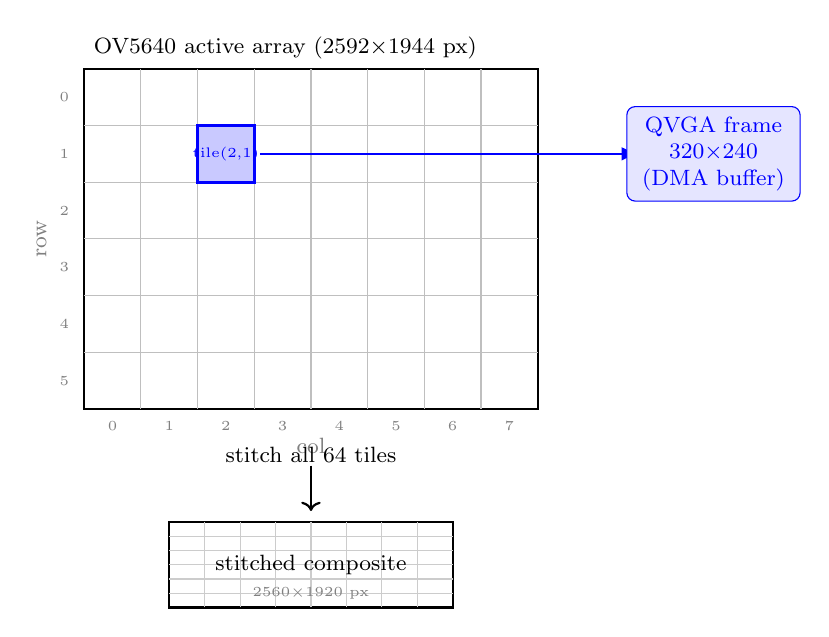
\begin{tikzpicture}[scale=0.72]
  % Outer sensor array border
  \draw[thick] (0,0) rectangle (8,6);
  \node[font=\footnotesize, anchor=south west] at (0,6) {OV5640 active array (2592$\times$1944 px)};

  % 8x8 grid lines
  \foreach \x in {1,...,7} { \draw[gray!50, thin] (\x,0) -- (\x,6); }
  \foreach \y in {1,...,5} { \draw[gray!50, thin] (0,\y) -- (8,\y); }

  % Highlight one tile (col=2, row=1 from top → y from bottom = 6-1-1=4)
  \fill[blue!30, opacity=0.7] (2,4) rectangle (3,5);
  \draw[blue, very thick] (2,4) rectangle (3,5);
  \node[font=\tiny, blue] at (2.5,4.5) {tile\\(2,1)};

  % Arrows showing col and row labels
  \foreach \c in {0,...,7} {
    \node[font=\tiny, gray] at (\c+0.5, -0.3) {\c};
  }
  \foreach \r in {0,...,5} {
    \node[font=\tiny, gray] at (-0.35, 5.5-\r) {\r};
  }
  \node[font=\footnotesize, gray] at (4,-0.65) {col};
  \node[font=\footnotesize, gray, rotate=90] at (-0.75,3) {row};

  % Arrow to captured tile and label
  \draw[-{Latex}, blue, thick] (3.1, 4.5) -- (9.8, 4.5);
  \node[draw, blue, rounded corners=3pt, fill=blue!10, minimum width=2.2cm,
        minimum height=1.2cm, font=\footnotesize, align=center]
        at (11.1, 4.5) {QVGA frame\\320$\times$240\\(DMA buffer)};

  % Stitched result below
  \draw[thick, ->] (4, -1.0) -- (4, -1.8);
  \node[font=\footnotesize] at (4, -0.8) {stitch all 64 tiles};
  \draw[thick] (1.5,-3.5) rectangle (6.5,-2.0);
  \foreach \x in {1,...,7} { \draw[gray!40,thin] (1.5+\x*5/8,-3.5) -- (1.5+\x*5/8,-2.0); }
  \foreach \y in {1,...,5} { \draw[gray!40,thin] (1.5,-2.0-\y*1.5/6) -- (6.5,-2.0-\y*1.5/6); }
  \node[font=\footnotesize] at (4,-2.75) {stitched composite};
  \node[font=\tiny, gray] at (4,-3.25) {2560$\times$1920 px};
\end{tikzpicture}
\caption{Tiled capture strategy.  The OV5640 sensor crop window (registers
  \texttt{0x3800}--\texttt{0x3807}) is repositioned for each of the
  $8\times 8 = 64$ tiles.  Each tile is captured as a QVGA JPEG into the
  fixed DRAM buffer; the ISP scales the crop to 320$\times$240.  The host
  stitches the tiles into a 2560$\times$1920 composite.}
\label{fig:tiling}
\end{figure}

\subsubsection{Bugs Identified and Planned Fixes}

During testing the system successfully captures the first tile but returns a
firmware error (HTTP 500) on every subsequent tile.  Two bugs in
\texttt{camera.c} and \texttt{server.c} were identified as the root causes.

\paragraph{Bug 1 --- \texttt{camera\_reset\_window()} calls \texttt{set\_framesize()},
breaking DMA synchronisation.}

After each tile capture, \texttt{camera\_reset\_window()} was implemented as:

\begin{verbatim}
s->set_framesize(s, s_cfg.frame_size);
\end{verbatim}

\texttt{set\_framesize()} rewrites a full set of OV5640 timing registers,
including subsampling (\texttt{0x3814}/\texttt{0x3815}) and binning
(\texttt{0x3820}/\texttt{0x3821}).  These register values determine the DVP
pixel-clock count per line.  The LCD\_CAM DMA controller was configured at
\texttt{esp\_camera\_init()} for the QVGA pixel-clock cadence; after
\texttt{set\_framesize()} changes those registers, the DMA loses sync and
\texttt{esp\_camera\_fb\_get()} returns \texttt{NULL} on the next call (tile 2
onwards).  Tile 1 succeeds because \texttt{camera\_reset\_window()} runs
\emph{after} the first capture completes and the damage only manifests on the
next \texttt{fb\_get()}.

\textbf{Fix:} replace the \texttt{set\_framesize()} call with direct register
writes that restore only the eight crop-window registers
(\texttt{0x3800}--\texttt{0x3807}) to their original values.  The original
values are read and saved on the first call to \texttt{camera\_set\_window()}
before any register is modified:

\begin{verbatim}
// Saved on first call to camera_set_window()
static bool    s_orig_window_saved = false;
static uint8_t s_orig[8]; // one entry per register 0x3800-0x3807
// masks matching those used in set_window
static const int s_masks[8] = {0x0F,0xFF,0x07,0xFF,0x0F,0xFF,0x07,0xFF};

// In camera_set_window(), before writing:
if (!s_orig_window_saved) {
    for (int i = 0; i < 8; i++)
        s_orig[i] = (uint8_t)s->get_reg(s, 0x3800+i, s_masks[i]);
    s_orig_window_saved = true;
}

// In camera_reset_window():
if (s_orig_window_saved)
    for (int i = 0; i < 8; i++)
        s->set_reg(s, 0x3800+i, s_masks[i], s_orig[i]);
\end{verbatim}

This restores the original crop window without touching subsampling,
binning, or any other register the DMA depends on.

\paragraph{Bug 2 --- No warm-up frame discarded after crop-window register write.}

The OV5640 applies I2C (SCCB) register writes at the next VSYNC boundary
(shadow-register mechanism).  At 30\,fps the inter-VSYNC period is $\sim$33\,ms;
the eight SCCB writes in \texttt{camera\_set\_window()} complete in
$\sim$4\,ms.  If a VSYNC occurs while the writes are in progress, or if the DMA
has already begun filling the buffer when \texttt{camera\_set\_window()} returns,
the very next \texttt{esp\_camera\_fb\_get()} call may return a frame captured
from the \emph{previous} crop window.

\textbf{Fix:} discard one frame immediately after \texttt{camera\_set\_window()}
returns, before the real tile capture:

\begin{verbatim}
camera_set_window(x, y, tile_w, tile_h);

// Discard one frame so the new crop window is guaranteed active.
camera_fb_t *warmup = esp_camera_fb_get();
if (warmup) esp_camera_fb_return(warmup);

camera_fb_t *fb = camera_capture_frame(); // real tile
camera_reset_window();
\end{verbatim}


% ─────────────────────────────────────────────────────────────────
\section{Verification}
% ─────────────────────────────────────────────────────────────────

\subsection{Servo Reliability and Repeatability Testing}

\subsubsection{Test Setup}

To characterise servo repeatability before integrating the gimbals into the
projection subsystem, a bench test was performed:

\begin{enumerate}
  \item A reference angle $\theta_{\text{ref}}$ was selected within the servo's
        operating range.
  \item The servo was commanded to $\theta_{\text{ref}}$, held for a fixed dwell
        period, then driven to a \emph{reset} position sufficiently far away to
        require a full-range movement on the return.
  \item The servo was commanded back to $\theta_{\text{ref}}$ and the final
        shaft position was measured.
  \item Steps 2--3 were repeated for $N$ trials ($N \approx 30$--50).
\end{enumerate}

Shaft position was recorded using \ldots

\begin{figure}[H]
  \centering
  \fbox{\parbox{0.7\textwidth}{\centering\vspace{2cm}
    \textit{[PLACEHOLDER: Diagram of servo test bench setup]}
  \vspace{2cm}}}
  \caption{Servo repeatability test bench.}
  \label{fig:servo_bench}
\end{figure}

Across repeated actuation trials, the servo returned to $\theta_{\text{ref}}$
with a maximum observed positional error of less than 1\,cm at a projection
distance of 3\,m.  The system accuracy requirement is $\pm 5$\,cm at the wall
surface, so this result is well within the required margin.

At 3\,m projection distance, a 1\,cm wall-surface error corresponds to an
angular error of:

\begin{equation}
  \Delta\theta = \arctan\!\left(\frac{0.01\;\text{m}}{3\;\text{m}}\right)
               \approx 0.19°
  \label{eq:angle_budget}
\end{equation}

The $\pm 5$\,cm requirement corresponds to $\approx 0.95°$ at the same distance,
giving a margin of $4\times$ on the servo repeatability alone, before any
closed-loop correction is applied.

\subsection{Servo Drive Tuning Verification}

Jerk and overshoot were assessed qualitatively before and after tuning by
observing the laser spot trajectory on a blank wall.  Before tuning the spot
exhibited a clear overshoot-and-return oscillation lasting approximately
[PLACEHOLDER]\,ms after each slew command.  After tuning with the fade + hold
profile described in Section~2.4, the oscillation was eliminated and settling
time was reduced to [PLACEHOLDER]\,ms.


\subsection{Tiled Capture Validation \textnormal{\textit{(pending bug fixes)}}}

Full end-to-end validation of the $8 \times 8$ tiled capture is blocked by the
two firmware bugs described in Section~2.6.3.  The first tile (col=0, row=0) is
captured and returned correctly, confirming that the endpoint routing, JSON
parsing, SCCB register writes, and JPEG response path are all functional.
Capture fails with HTTP~500 on every tile after the first because
\texttt{camera\_reset\_window()} corrupts the DMA state via \texttt{set\_framesize()}.

Once the fixes are applied --- replacing \texttt{set\_framesize()} with direct
register restoration and adding a warm-up frame discard --- the planned
validation procedure is:

\begin{enumerate}
  \item Execute a full $8 \times 8$ sequence against a wall target with a
        printed grid of known geometry.
  \item Inspect each tile for correct content (no repeated or shifted frames).
  \item Stitch the tiles using \texttt{client.py capture-tiled} and measure
        seam registration error between adjacent tiles.
  \item Compare the stitched composite to a reference image taken from closer
        range to confirm the full sensor area is covered.
\end{enumerate}

\begin{figure}[H]
  \centering
  \fbox{\parbox{0.7\textwidth}{\centering\vspace{2.5cm}
    \textit{[PLACEHOLDER: Stitched $2560\times1920$ composite image of the
    climbing wall / test target --- to be captured after bug fixes]}
  \vspace{2.5cm}}}
  \caption{Stitched composite from a full $8\times 8$ tiled capture (pending).}
  \label{fig:stitched}
\end{figure}

% ─────────────────────────────────────────────────────────────────
\section{Conclusion}
% ─────────────────────────────────────────────────────────────────

\subsection{Summary}

My individual work has spanned hardware, firmware, and vision software across
the BetaSpray system.  The key deliverables to date are:

\begin{enumerate}
  \item A fabricated two-layer PCB with a correctly sized servo power rail and
        bulk capacitance, based on a quantitative transient analysis.
  \item A working servo firmware driver with a tuned fade/hold profile that
        meets the mechanical settling requirements.
  \item Servo reliability data quantifying position variability relative to the
        $\pm 5$\,cm system requirement.
  \item Camera calibration tooling and a lens-distortion model integrated into
        the firmware build.
  \item A tiled high-resolution capture pipeline (in progress) targeting
        $2560\times1920$ stitched images from the memory-constrained N8 dev
        board; two firmware bugs identified and fixes planned, with full
        validation targeted for 2026-04-10.
\end{enumerate}

\subsection{Timeline and Remaining Work}

\begin{table}[H]
  \centering
  \caption{Remaining milestones.}
  \label{tab:timeline}
  \begin{tabular}{lll}
    \toprule
    Task & Target Date & Status \\
    \midrule
    Validate tiled stitching on climbing wall & 2026-04-10 & In Progress \\
    Integrate DoG detector with tiled input & April 2026 & Planned \\
    Closed-loop laser spot correction & April 2026 & Planned \\
    Full system demo & May 2026 & Planned \\
    Final report & May 2026 & Planned \\
    \bottomrule
  \end{tabular}
\end{table}

\subsection{Ethical Considerations}

The BetaSpray system uses low-power Class~II laser modules directed at a
climbing wall.  Direct exposure to the laser beam poses an eye hazard.  Mitigations
include:

\begin{itemize}
  \item Software limits on servo range to prevent the laser from pointing
        outside the designated wall area.
  \item A hardware \texttt{/stop} endpoint that immediately disables all servo
        PWM output.
  \item Physical shielding of the gimbal assembly during operation to prevent
        accidental beam scatter.
\end{itemize}

The system processes wall images on-device and transmits only hold coordinate
lists and compressed JPEG frames over a local Wi-Fi network (no cloud
connection), minimising any privacy surface.

% ─────────────────────────────────────────────────────────────────
\begin{thebibliography}{9}

\bibitem{ov5640}
OmniVision Technologies, ``OV5640 5-Megapixel (2592$\times$1944) CMOS Image
Sensor,'' Application Note, 2013.

\bibitem{sg90}
TowerPro, ``SG90 9g Micro Servo,'' Datasheet, 2010.

\bibitem{lm3940}
Texas Instruments, ``LM3940 1-A Low-Dropout Regulator for 5-V to 3.3-V
Conversion,'' SNVS034E, 2013.

\bibitem{opencv_calib}
G.~Bradski and A.~Kaehler, \textit{Learning OpenCV: Computer Vision with the
OpenCV Library}. O'Reilly Media, 2008.

\bibitem{brown_conrady}
D.~C.~Brown, ``Decentering Distortion of Lenses,'' \textit{Photometric
Engineering}, vol.~32, pp.~444--462, 1966.

\bibitem{espidf}
Espressif Systems, ``ESP-IDF Programming Guide,'' v5.x,
\url{https://docs.espressif.com/projects/esp-idf/en/latest/}.

\end{thebibliography}

\end{document}
